\begin{center}
  \Large
  \textbf{BIOGRAFI PENULIS}
\end{center}

\addcontentsline{toc}{chapter}{BIOGRAFI PENULIS}

\vspace{2ex}

% [Foto penulis] Ganti dummy_image.jpg dengan foto close-up 4x6 cm
\begin{wrapfigure}{L}{0.3\textwidth}
  \centering
  \vspace{-3ex}
  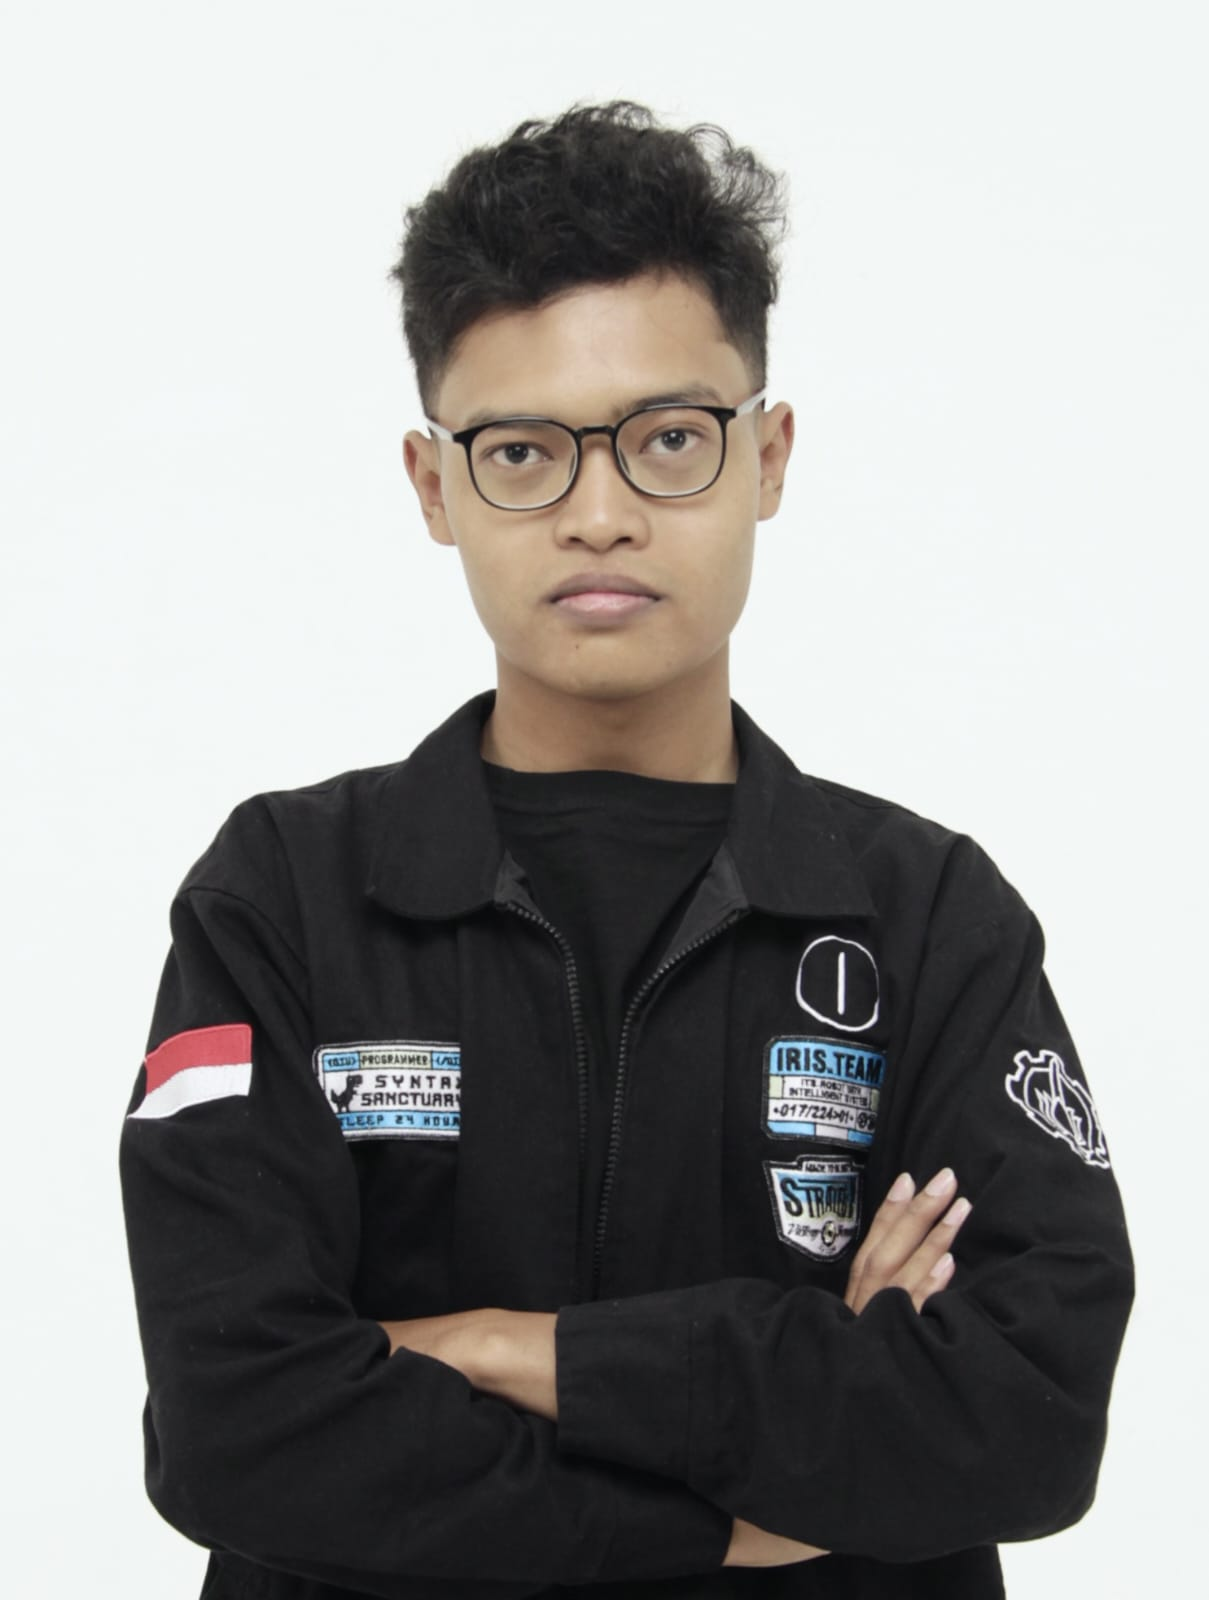
\includegraphics[width=0.3\textwidth]{gambar/foto_hernanda.jpeg}
  \vspace{-4ex}
\end{wrapfigure}

Penulis bernama Hernanda Achmad Priyatna dengan NRP 5022221114.
Penulis menempuh pendidikan di Departemen Teknik Elektro, Fakultas Teknologi Elektro dan Informatika Cerdas, Institut Teknologi Sepuluh Nopember (ITS) Surabaya.

Sejak semester pertama, penulis aktif dalam Tim IRIS (\emph{ITS Robot with Intelligence System}) yaitu Tim Riset Robotika ITS yang berfokus pada pengembangan robot sepak bola beroda otonom untuk kompetisi internasional RoboCup Medium Size League sebagai divisi \emph{Programmer}.
Selama di IRIS, penulis mendalami bidang visi komputer, estimasi keadaan, sistem kendali, dan navigasi otonom.
Penulis juga mengikuti beberapa kompetisi robotika di tingkat nasional dan internasional bersama tim IRIS salah satunya adalah FIRA RoboWorldCup 2025 di Korea Selatan dengan memperoleh juara 1 \emph{All-Round Autonomous Cars Physical Pro}, juara 1 \emph{Race Category Autonomous Cars Physical Pro}, dan juara 2 \emph{Urban Category Autonomous Cars Physical Pro}.

Ketertarikan penulis pada robotika otonom membawa penulis pada topik
tugas akhir ini, yaitu navigasi mobil otonom menggunakan segmentasi
visual dan data GPS. Melalui penelitian ini, penulis mengembangkan
sistem navigasi berbasis persepsi visual dan fusi sensor pada
platform kendaraan listrik Omoda E5. Pengalaman tersebut membentuk
kemampuan teknis penulis dalam pengembangan perangkat lunak menggunakan
ROS2, pemrosesan citra, serta implementasi algoritma navigasi pada
sistem \emph{real-time}.
